\documentclass[12pt,a4paper]{article}
\usepackage[utf8]{inputenc}
\usepackage{graphicx}
\usepackage{tikz}
\usetikzlibrary{fit}
\usepackage{lmodern}
\usepackage{sectsty}

\sectionfont{\color{cyan}}
\begin{document}
   \begin{titlepage}
      {\fontfamily{lmss}\selectfont
          \centering
          
\includegraphics[width=0.40\textwidth]{logo.png}\par\vspace{1cm}
          {\LARGE CSIR \par}
          \vspace{0.25cm}
          {\huge\bfseries \color{cyan}Electronically Timing Athletes\par}
          \vspace{1cm}
          {\Large\textit{by} Brute Force\par}
         \vspace{0.25cm}
         \begin{tikzpicture}
            \node [inner sep=0pt,,outer sep=0pt,clip,rounded corners=0.5cm] (pict) at (0,0) {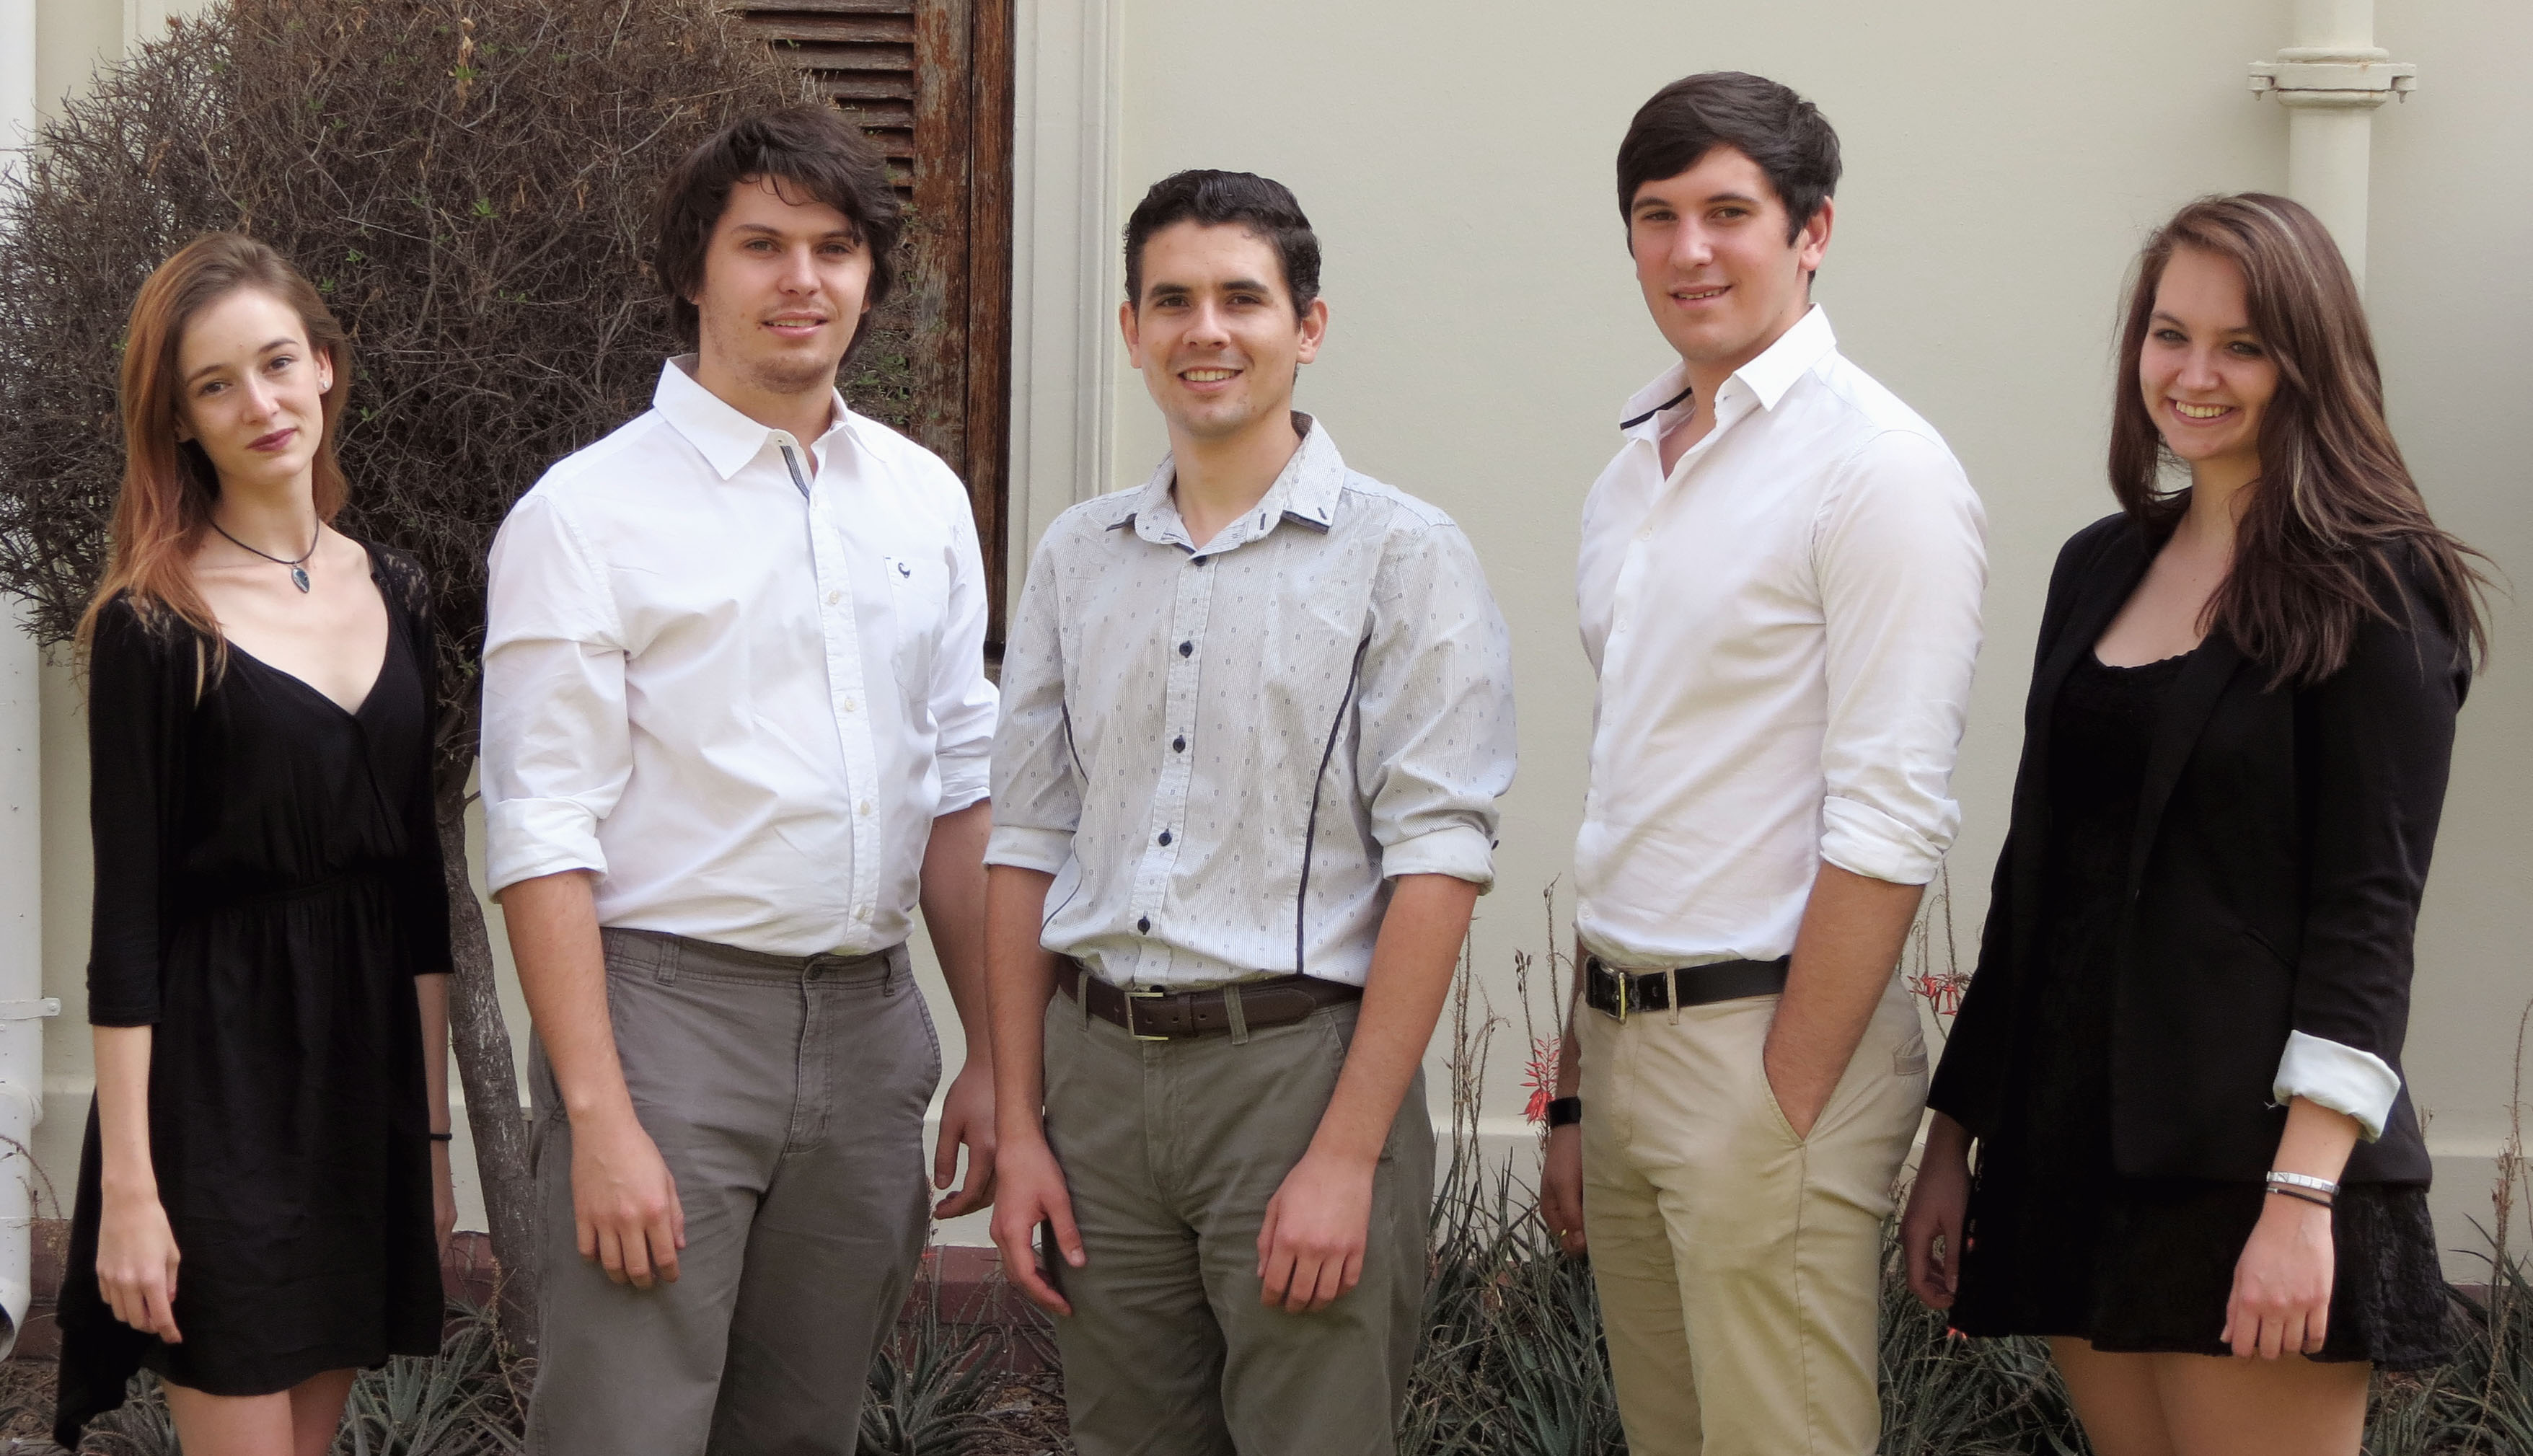
\includegraphics[width=0.9\textwidth]{team.jpg}};
            \node[fit=(pict),rounded corners=.55cm,inner sep=2pt]{};
         \end{tikzpicture}

         \par\vspace{1cm}
         \date{}
         \author{}
         \title{}
         \centering
         \textbf{Authors:}\\
         Mia Gerber\\
         Matthew Perry\\
         Wanrick Willemse\\
         Duart Breedt\\
         Linda Potgieter\\
      }
   \end{titlepage}
   \maketitle
   \tableofcontents
   \newpage
   
   \section{Project Description}
The project scope includes creating a RFID reader interface, storing timing and athlete data on a database when both online and offline, performing statistical analysis on database data, high Human Computer Interaction design standards when considering Graphical User Interface design, as well as successful registration of athletes.\\\\
The system will consist of technology to interface with the RFID reader provided by the client. We will only be able to decide on technology to interface with this reader when we have access to it. \\\\
Web Development technologies such as PHP, HTML, CSS, Bootstrap, JavaScript will be used to create a create a display that will be able to update in real time with data such as the current elapsed time and a number of athletes still participating. Any additional MEAN or LAMP stack technologies will be used as deemed necessary. The design of the web interface will be of utmost importance. The GUI will adhere to Human Computer Interaction Design principles to ensure effective use by the users.\\\\
For database functionalities, we will use SQL databases since there is no need for a great amount of handling of concurrent read and writes to the database. For Statistical analysis of the data, we will use math.js for calculations along with plot.js to visualise athlete relevant statistics based on the timing and distance data within the database. \\\\
We will design an interface which will be able to register an athlete to a specific RFID chip using a unique ID. Further registration specifics will depend on the design of the RFID and which data it can provide when read by the supplied reader.\\\\
When the RFID chip makes contact with the reader, data communication will be triggered. Details such as the athlete's unique ID and the exact time to finish the current race will be recorded and sent to either the online or the offline database. The unique ID is used in conjunction with the timing device data to ensure slow data transfer does not affect the recorded time.\\\\
A server will host this database to ensure real-time updating of the database. Server technologies will include MEAN Stack resources such as Node.js To ensure there is no data loss when there is no connection to the server (when the system is offline), data will be stored in a database. These data will then be uploaded to the database on the server as soon as there is an established connection between the two. As soon as the data are uploaded they will be removed from the offline database to prevent it from using unnecessary space. 


\subsection{Deployment Diagram}
\begin{center}
    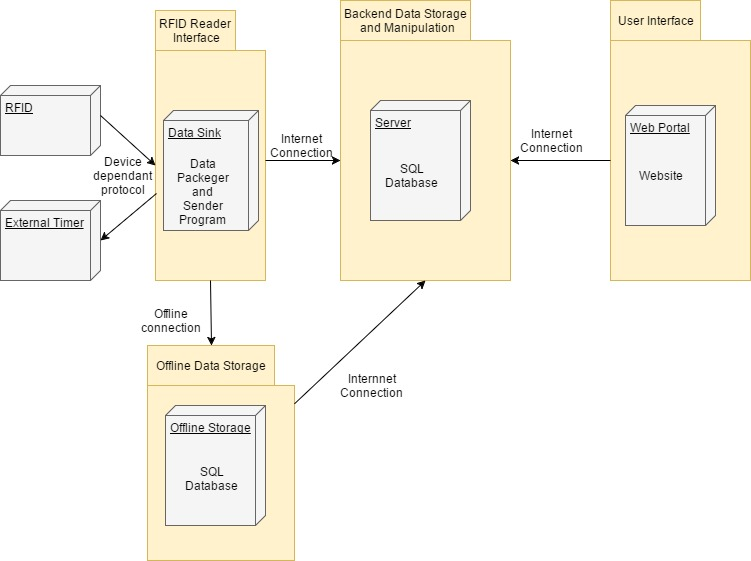
\includegraphics[width=0.5\linewidth]{ETADeployment.jpg}
\end{center}

\section{Development Methodologies}
\subsection{Interaction between development team and client}

\textnormal 
Involvement of the client is of utmost importance to ensure complete and on goal developed software. Client meetings will be arranged in advance with members of the team prepared with concerns and questions to ensure effective use of the client's time. 
As specified in the original project specifications provided by the client, the team will meet with the client either one week before, or one week after each major demonstration (dates of demonstrations as provided by the University of Pretoria COS 301 module). 
            \\ \\
            Moving more into the realm of software engineering, as a team we plan on strictly adhering 
            to Agile Principles. Clients will not only be queried for information but involved as much
            as possible in the testing of early prototypes so that their feedback can be integrated and 
            used as a guide for future releases.
            \\ \\
            Lastly, it is important to us that we as developers and you as our client at CSIR both 
            agree on a scope for the project, requirements can and probably will change but in order
            to provide the best quality product in the time-frame given we need to first create a checklist of features to be implemented and continually refer back to them to ensure we are not going off the scope.
                

\subsection{Interaction between members of development team}

\textnormal We decided on applying a SCRUM methodology in order to structure how teamwork will occur for
            this project, this is a faster, more intensely iterative approach to controlling workflow.
            We are using Slack and ZenHub (in conjunction with Github) to ensure that team members are aware of each other even when we are not physically together and are alerted when work is either available or completed.
            \\ \\
            Meetings will be held once a week regardless of whether there is a problem with the project or not, each meeting will require that each team member gives a small summary of what work they had done that week, this enforces accountability. Working in weekly "sprints" also optimises predictability and minimises risk (if something does go wrong it is only a week's worth of work lost, not a whole month)
            \\ \\
            As a team, we are going to be adhering to a practice called "pair-programming" which is essentially two or more people working on the same piece of code or feature in order to maximise the chances of bugs being discovered and minimise the time required to get a feature ready for production. \\\\
We will strictly follow the software development life cycle. 
Planning includes requirement and quality assurance analysis.   
The basic requirements have been provided, we have in this document defined and elaborated on them and their technologies. The client must approve these requirements and technologies.  \\\\
Once the client has given approval, we will start with designing the product architecture based on the requirements. This will clearly define all the architectural modules as well as its communication and data flow representation with the external and third party modules such as the external timing device and the RFID tags.  \\\\
After the design is complete, we will start with building the product using the agile methodology mentioned above. 
Testing will not be a once off phase, but instead, there will be continuous assessment of the product throughout the building process. Client input will be required for certain critical tests. \\\\
When the product is complete and complies with the team's high standards, it will be handed over to the CSIR for deployment. 
            \\ \\ 

    \newpage
    \section{Our Team}
       Team details here:
        \subsection{Mia Gerber}
        Short personal summary\\\\
        \textbf{\small Relevant skills:}
        \begin{itemize}
            \item skill 1
            \item skill 2
            \item skill 3
        \end{itemize}
        
        
        \subsection{Matthew Perry}
        Short personal summary\\\\
        \textbf{\small Relevant skills:}
        \begin{itemize}
            \item skill 1
            \item skill 2
            \item skill 3
        \end{itemize}
        
        \subsection{Wanrick Willemse}
        Short personal summary\\\\
        \textbf{\small Relevant skills:}
        \begin{itemize}
            \item skill 1
            \item skill 2
            \item skill 3
        \end{itemize}
        
    
        \subsection{Duart Breedt}
        Short personal summary\\\\
        \textbf{\small Relevant skills:}
        \begin{itemize}
            \item skill 1
            \item skill 2
            \item skill 3
        \end{itemize}
        
        
        \subsection{Linda Potgieter}
        Short personal summary\\\\
        \textbf{\small Relevant skills:}
        \begin{itemize}
            \item skill 1
            \item skill 2
            \item skill 3
        \end{itemize}

\end{document}
